\chapter{The best students, where do they study? A rating case study}
\label{sec:14}

\abstract*{In 2004, the German magazine \emph{Der Spiegel}, with the help of \emph{McKinsey \& Company} and \emph{AOL}, conducted an extensive online survey, assessing the apparent quality of German University students Footnote[28]. More than 80,000 students, by participating, were questioned on their '\emph{Abitur}' and university exams' marks, time of studies and age, grants, awards and publications, IT proficiency, linguistic skills, practical work experience, foreign mobility and civil engagement. Each student received in return a quality score through a specific weighing of the collected data which depended on the subject the student is mainly studying. \footnote{The methology (in German) guiding the \emph{Spiegel} survey may be consulted in the \texttt{examples} directory of the \Digraph resources.}. The eventually published results by the \emph{Spiegel} magazine concerned nearly 50,000 students, enroled in one of fifteen popular academic subjects, like \emph{German Studies}, \emph{Life Sciences}, \emph{Psychology}, \emph{Law}  or \emph{CS}. Publishing only those subject-University combinations, where at least 18 students had correctly filled in the questionnaire, left 41 German Universities where, for at least eight out of the fifteen subjects, an average enrolment quality score could be determined. Based on this published data Footnote[28], we present and discuss in this chapter, how to \emph{rate} with the help of our \Digraph software ressources the apparent global \emph{enrolment quality} of these 41 higher education institutions.}

\abstract{In 2004, the German magazine \emph{Der Spiegel}, with the help of \emph{McKinsey \& Company} and \emph{AOL}, conducted an extensive online survey, assessing the apparent quality of German University students Footnote[28]. More than 80,000 students, by participating, were questioned on their '\emph{Abitur}' and university exams' marks, time of studies and age, grants, awards and publications, IT proficiency, linguistic skills, practical work experience, foreign mobility and civil engagement. Each student received in return a quality score through a specific weighing of the collected data which depended on the subject the student is mainly studying. \footnote{The methology (in German) guiding the \emph{Spiegel} survey may be consulted in the \texttt{examples} directory of the \Digraph resources.}. The eventually published results by the \emph{Spiegel} magazine concerned nearly 50,000 students, enroled in one of fifteen popular academic subjects, like \emph{German Studies}, \emph{Life Sciences}, \emph{Psychology}, \emph{Law}  or \emph{CS}. Publishing only those subject-University combinations, where at least 18 students had correctly filled in the questionnaire, left 41 German Universities where, for at least eight out of the fifteen subjects, an average enrolment quality score could be determined. Based on this published data Footnote[28], we present and discuss in this chapter, how to \emph{rate} with the help of our \Digraph software ressources the apparent global \emph{enrolment quality} of these 41 higher education institutions.}

\section{The performance tableau}
\label{sec:14.1}

Published data of the 2004 \emph{Spiegel} student survey is stored, for our evaluation purpose here, in a file named \texttt{studentenSpiegel04.py} of \texttt{PerformanceTableau} format \footnote{The performance tableau \texttt{studentenSpiegel04.py} is also available in the \texttt{examples} directory of the \Digraph software collection.}.

\begin{lstlisting}[caption={The 2004 Spiegel students survey data},label=list:14.1]
>>> from perfTabs import PerformanceTableau
>>> t = PerformanceTableau('studentenSpiegel04')
>>> t
  *------- PerformanceTableau instance description -*
    Instance class    : PerformanceTableau
    Instance name     : studentenSpiegel04
    Actions           : 41 (Universities)
    Criteria          : 15 (academic subjects)
    NA proportion (%) : 27.3
    Attributes        : ['name', 'actions',
                         'objectives', 'criteria',
                         'weightPreorder',
                         'evaluation']
>>> t.showHTMLPerformanceHeatmap(ndigits=1,\
...                              rankingRule=None)
\end{lstlisting}

\begin{figure}[h]
%\sidecaption
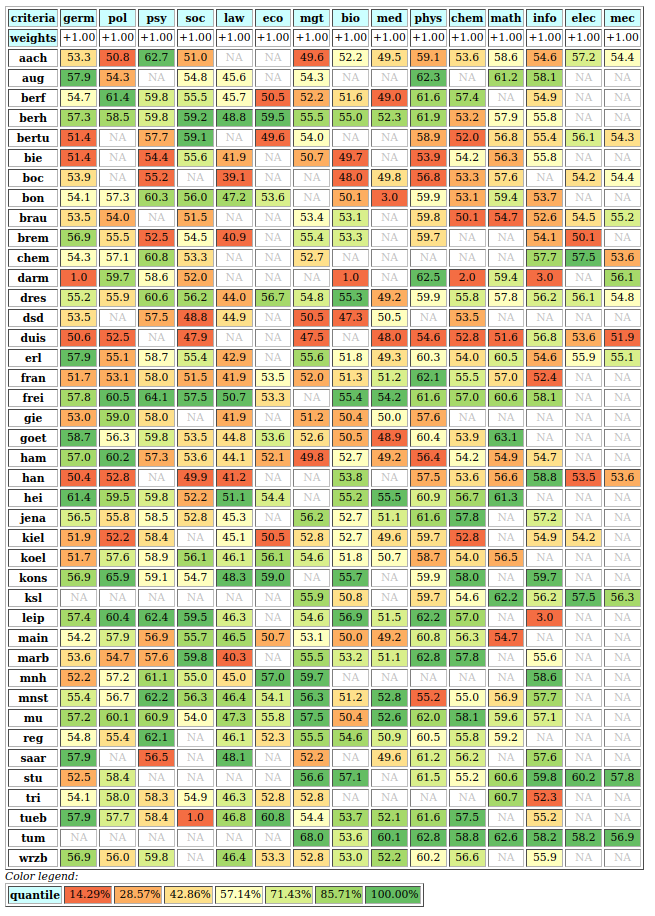
\includegraphics[width=12cm]{Figures/ratingData.png}
\caption{Average quality of enroled students per academic subject}
\label{fig:14.1}       % Give a unique label
\end{figure}
\clearpage
In Fig. \ref{fig:14.1}, the fifteen popular academic subjects are grouped into topical 'Faculties': - \emph{Humanities}; - \emph{Law, Economics \& Management}; - \emph{Life Sciences \& Medicine}; - \emph{Natural Sciences \& Mathematics}; and - \emph{Technology}. All fifteen subjects are considered equally significant for our evaluation problem (see Row 2). The recorded average enrolment quality scores appear coloured along a 7-tiling scheme per subject (see last Row).

We may by the way notice that TU Dresden is the only Institution showing enrolment quality scores in all the fifteen academic subjects. Whereas, on the one side, TU Muenchen and Kaiserslautern are only valuated in \emph{Sciences} and \emph{Technology} subjects. On the other side, Mannheim, is only valuated in \emph{Humanities} and \emph{Law, Economics \& Management} studies. Most of the 41 Universities are not valuated in \emph{Engineering} studies. We are, hence, facing a large part ($27.3\%$) of irreducible missing data (see Listing \ref{list:14.1} Line 9 and Chapter \ref{sec:16} coping with missing data).

Details of the enrolment quality criteria (the academic subjects) may be consulted in a browser view (see :numref:`spiegelCriteria` below).

\begin{lstlisting}
>>> t.showHTMLCriteria()
\end{lstlisting}
 
\begin{figure}[h]
%\sidecaption
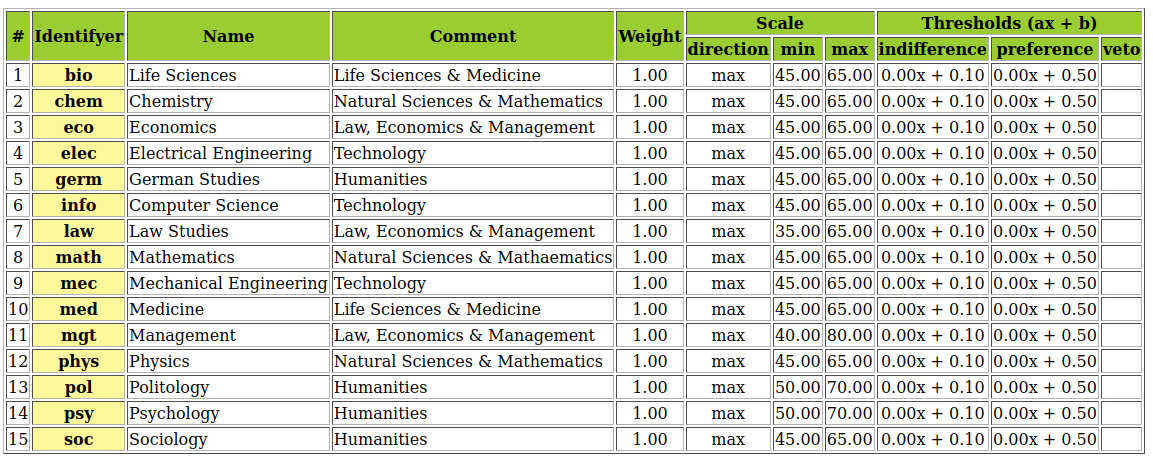
\includegraphics[width=12cm]{Figures/spiegelCriteria.png}
\caption{Details of the rating criteria}
\label{fig:14.2}       % Give a unique label
\end{figure}
%\clearpage
The evaluation of the individual quality score for a participating student actually depends on his or her mainly enroled subject \footnote{The methology (in German) guiding the \emph{Spiegel} survey may be consulted in the \texttt{examples} directory of the \Digraph resources.}. The apparent quality measurement scales thus largely differ indeed from subject to subject (see Fig. \ref{fig:14.2}), like \emph{Law Studies} ($35.0 - 65-0$) and \emph{Politology} ($50.0 - 70.0$). The recorded average enrolment quality scores, hence, are in fact \emph{incommensurable} between the subjects.

To take furthermore into account a potential and very likely imprecision of the individual quality scores' computation, we shall assume that, for all subjects, an average enrolment quality score difference of $0.1$ is \emph{insignificant}, wheras a difference of $0.5$ is sufficient to positively attest a \emph{better} enrolment quality.

The apparent incommensurability and very likely imprecision of the recorded average enrolment quality scores, renders meaningless any global averaging over the subjects per University of the enrolment quality. We shall therefore, similarly to the methodological approach of the \emph{Spiegel} authors, proceed with an \emph{order statistics} based rating-by-ranking approach (see Chapter \ref{sec:10} on rating with learned quantile norms).

\section{Rating-by-ranking with lower-closed quantile limits}
\label{sec:14.1}

The \emph{Spiegel} authors opted indeed for a simple 3-tiling of the Universities per valuated academic subject, followed by an average \Borda scores based global ranking. Here, our epistemic logic based outranking approach, allows us, with adequate choices of \emph{indifference} ($0.1$) and \emph{preference} ($0.5$) discrimination thresholds, to estimate \emph{lower-closed} 9-tiles of the enrolment quality scores per subject and rank conjointly, with the help of the \Copeland ranking rule Footnote[34] applied to a corresponding bipolar-valued outranking digraph, the 41 Universities \textbf{and} the lower limits of the estimated 9-tiles limits.

First, we therefore need, with the help of the \texttt{PerformanceQuantiles} constructor, to estimate the lowerclosed 9-tiling of the average enrolment quality scores per academic subject.

\begin{lstlisting}[caption={Computing 9-tiles of the enrolment quality scores per subject},label=list:14.2]
>>> from performanceQuantiles import PerformanceQuantiles
>>> pq = PerformanceQuantiles(t,numberOfBins=9,LowerClosed=True)
>>> pq
  *------- PerformanceQuantiles instance description ------*
    Instance class   : PerformanceQuantiles
    Instance name    : 9-tiled_performances
    Criteria         : 15
    Quantiles        : 9 (LowerClosed)
    History sizes    : {
      'germ': 39, 'pol': 34, 'psy': 34, 'soc': 32,
      'law': 32, 'eco': 21, 'mgt': 34,
      'bio': 34, 'med': 28, 'phys': 37, 'chem': 35, 'math': 27,
      'info': 33, 'elec': 14, 'mec': 13,}
\end{lstlisting}

The history sizes, reported in Listing \ref{list:14.2} above, indicate the number of Universities valuated in each one of the popular fifteen subjects. \emph{German Studies}, for instance, are valuated for 39 out of 41 Universities, whereas \emph{Electrical} and \emph{Mechanical Engineering} are only valuated for 14, respectively 13 Institutions. None of the fifteen subjects are valuated in all the 41 Universities \footnote{It would have been much more accurate to estimate such quantile limits from the individual qualitiy scores of all the nearly 50,000 surveyed students. But this data was not public.}. 

We may inspect the resulting 9-tiling limits in a browser view.

\begin{lstlisting}
>>> pq.showHTMLLimitingQuantiles(Transposed=True,Sorted=False,\
...	   ndigits=1,title='9-tiled quality score limits')
\end{lstlisting}

\begin{figure}[h]
\sidecaption
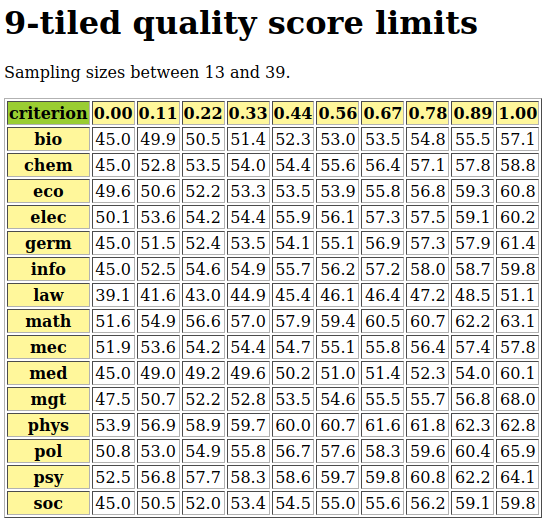
\includegraphics[width=7cm]{Figures/score9Limits.png}
\caption{9-tiling quality score limits per academic subject. We see confirmed again the incommensurability between the subjects, we noticed already in the apparent enrolment quality scoring , especially between \emph{Law Studies} ($39.1 - 51.1$) and \emph{Politology} ($50.5 - 65.9$). Universities valuated in \emph{Law studies} but not in \emph{Politology}, like the University of Bielefeld, would see their enrolment quality unfairly weakened when simply averaging the enrolment quality scores over valuated subjects}
\label{fig:14.3}       % Give a unique label
\end{figure}
%\clearpage
We add, now, these 9-tiling quality score limits to the enrolment quality records of the 41 Universities and rank all these records conjointly together with the help of the \texttt{LearnedQuantilesRatingDigraph} constructor and by using the \Copeland ranking rule.

\begin{lstlisting}
>>> from sortingDigraphs import\
...                 LearnedQuantilesRatingDigraph
>>> lqr = LearnedQuantilesRatingDigraph(pq,t,\
...                 rankingRule='Copeland')
\end{lstlisting}

The resulting ranking of the 41 Universities including the lower-closed 9-tiling score limits may be nicely illustrated  with the help of a corresponding heatmap view . 

\begin{lstlisting}
>>> lqr.showHTMLRatingHeatmap(colorLevels=7,\
...              Correlations=True,\
...              ndigits=1,rankingRule='Copeland')
\end{lstlisting}

\begin{figure}[h]
%\sidecaption
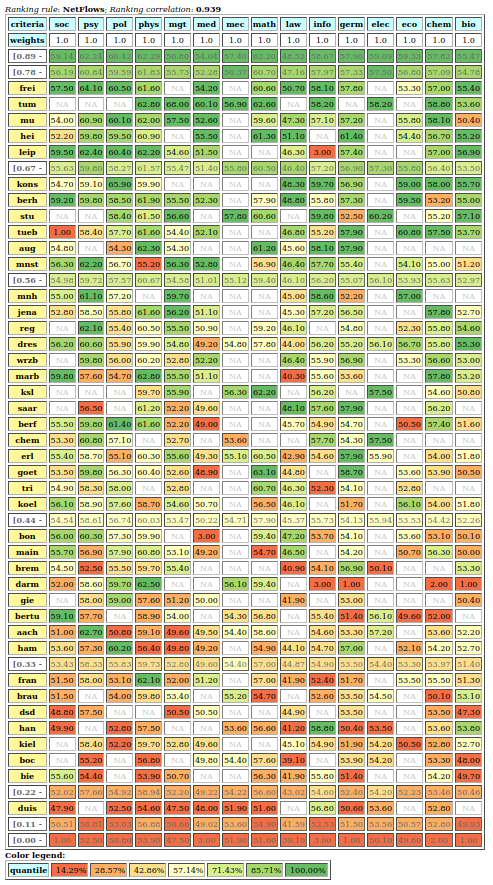
\includegraphics[width=11cm]{Figures/nineTilingResult.png}
\caption{Heatmap view of the 9-tiles rating-by-ranking result}
\label{fig:14.4}       % Give a unique label
\end{figure}
%\clearpage
The ordinal correlation ($+0.967$) Footnote[35] of the \Copeland ranking with the underlying bipolar-valued outranking digraph is very high (see Fig. \ref{fig:14.4} Row 1). Most correlated subjects with this rating-by-ranking result appear to be \emph{German Studies} ($+0.51$), \emph{Chemistry} ($+0.48$), \emph{Management} ($+0.47$) and \emph{Physics} ($+0.46$). Both \emph{Electrical} ($+0.07$) and \emph{Mechanical Engineering} ($+0.05$) are the less correlated subjects (see Row 3).

From the actual ranking position of the lower 9-tiling limits, we may now immediately deduce the 9-tile enrolment quality equivalence classes. No University reaches the highest 9-tile ($[0.89 - [$). In the lowest 9-tile ($[0.00- 0.11]$) we find the University Duisburg. The complete rating result may be easily printed out as follows.

\begin{lstlisting}[caption={Computing 9-tiles of the enrolment quality scores per subject},label=list:14.3]
>>> lqr.showQuantilesRating()
    *-------- Quantiles rating result ---------
     [0.89 - 1.00] []
     [0.78 - 0.89[ ['tum','frei','kons','leip','mu','hei']
     [0.67 - 0.78[ ['stu','berh']
     [0.56 - 0.67[ ['aug','mnh','tueb','mnst','jena',
                    'reg','saar']
     [0.44 - 0.56[ ['wrzb','dres','ksl','marb','berf',
                    'chem','koel','erl','tri']
     [0.33 - 0.44[ ['goet','main','bon','brem']
     [0.22 - 0.33[ ['fran','ham','kiel','aach',
                    'bertu','brau','darm']
     [0.11 - 0.22[ ['gie','dsd','bie','boc','han']
     [0.00 - 0.11[ ['duis']
\end{lstlisting}

Following Universities: TU München, Freiburg, Konstanz, Leipzig, München as well as Heidelberg, appear best rated in the eigth 9-tile ($[0.78 - 0.89[$, see Listing \ref{list:14.3} Line 4). Lowest-rated in the first 9-tile, as mentioned before, appears University Duisburg (Line 14). Midfield, the fifth 9-tile ($[0.44 - 0.56[$), consists of the Universities Würzburg, TU Dresden, Kaiserslautern, Marburg, FU Berlin, Chemnitz, Köln , Erlangen-Nürnberg and Trier (Lines 8-9).

A corresponding \emph{graphviz} drawing may well illustrate all these enrolment quality equivalence classes.

\begin{lstlisting}
>>> lqr.exportRatingByRankingGraphViz(fileName='ratingResult',\
...                                   graphSize='12,12')
  *---- exporting a dot file for GraphViz tools ---------*
   Exporting to ratingResult.dot
   dot -Grankdir=TB -Tpdf dot -o ratingResult.png
\end{lstlisting}

\begin{figure}[h]
%\sidecaption
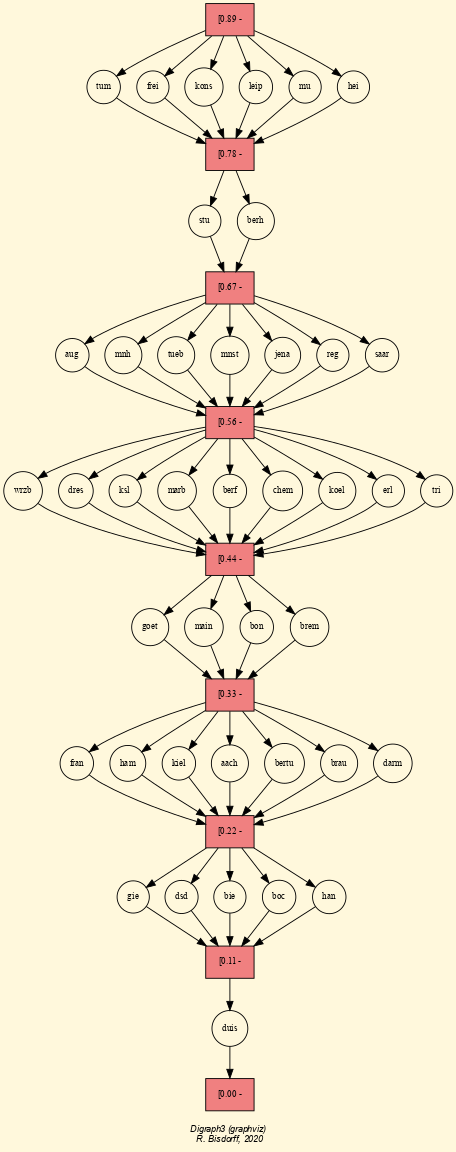
\includegraphics[width=7cm]{Figures/ratingResult.png}
\caption{Drawing of the 9-tiles rating-by-ranking result}
\label{fig:14.5}       % Give a unique label
\end{figure}
%\clearpage

% \begin{lstlisting}[caption={Epistemic fusion of Copeland and Netflows rating-by-ranking results},label=list:14.5]
% >>> lqr = LearnedQuantilesRatingDigraph(\
% ...           pq,t,rankingRule='Copeland')
% >>> lqr1 = LearnedQuantilesRatingDigraph(\
% ...           pq,t,rankingRule='NetFlows')
% >>> from transitiveDigraphs import\
% ...           RankingsFusionDigraph
% >>> rankings = [lqr.actionsRanking, \
% ...           lqr1.actionsRanking]
% >>> rf = RankingsFusionDigraph(lqr,rankings)
% >>> rf.exportGraphViz(fileName='fusionResult',\
% ...           WithRatingDecoration=True,\
% ...           graphSize='30,30')
%   exporting a dot file for GraphViz tools
%    Exporting to fusionResult.dot
%    dot -Grankdir=TB -Tpng fusionResult.dot\
% ...                  -o fusionResult.png
% \end{lstlisting}

\begin{minipage}{7cm}
\textbf{Fig. 14.6} Fused Copeland and NetFlows ratings

\noindent We have noticed in Chapter 8 \ref{sec:8}, that there is not a single optimal rule for ranking from a given outranking digraph. The \Copeland rule, for instance, has the advantage of being \Condorcet consistent, i.e. when the outranking digraph models in fact a linear ranking, this ranking will necessarily be the result of the \Copeland* rule. When this is not the case, and especially when the outranking digraph shows many circuits, all potential ranking rules may give very divergent ranking results, and hence also substantially divergent rating-by-ranking results.

It is, hence, interesting, to verify if the epistemic fusion of the rating-by-ranking results, one may obtain when applying two different ranking rules, like the \Copeland and the \NetFlows ranking rule, does actually confirm our rating-by-ranking result shown in Fig. \ref{fig:14.5}. For this purpose we make usage of the \texttt{RankingsFusionDigraph} constructor (see Line 9 below).

{\scriptsize
\begin{verbatim}
>>> lqr = LearnedQuantilesRatingDigraph(\
...           pq,t,rankingRule='Copeland')
>>> lqr1 = LearnedQuantilesRatingDigraph(\
...           pq,t,rankingRule='NetFlows')
>>> from transitiveDigraphs import\
...           RankingsFusionDigraph
>>> rankings = [lqr.actionsRanking, \
...           lqr1.actionsRanking]
>>> rf = RankingsFusionDigraph(lqr,rankings)
>>> rf.exportGraphViz(fileName='fusionResult',\
...           WithRatingDecoration=True,\
...           graphSize='30,30')
  exporting a dot file for GraphViz tools
   Exporting to fusionResult.dot
   dot -Grankdir=TB -Tpng fusionResult.dot\
...                  -o fusionResult.png
\end{verbatim}
}
  
In the Figure here, we notice that many Universities appear now rated into several adjacent 9-tiles. The previously best-rated Universities: TU München, Freiburg, München, Leipzig, as well as  Heidelberg, for instance, appear now sorted into the $7^{th}$ and $8^{th}$ 9-tile ($[0.67 - 0.89]$), whereas Konstanz is now, even more imprecisely, rated into the $6^{th}$, the $7^{th}$ and the $8^{th}$ 9-tile.

How confident, hence, is our precise Copeland rating-by-ranking result? To investigate this question, let us now inspect the outranking digraph on which we actually apply the \Copeland ranking rule.

\end{minipage}
\begin{minipage}{4cm}
\begin{center}
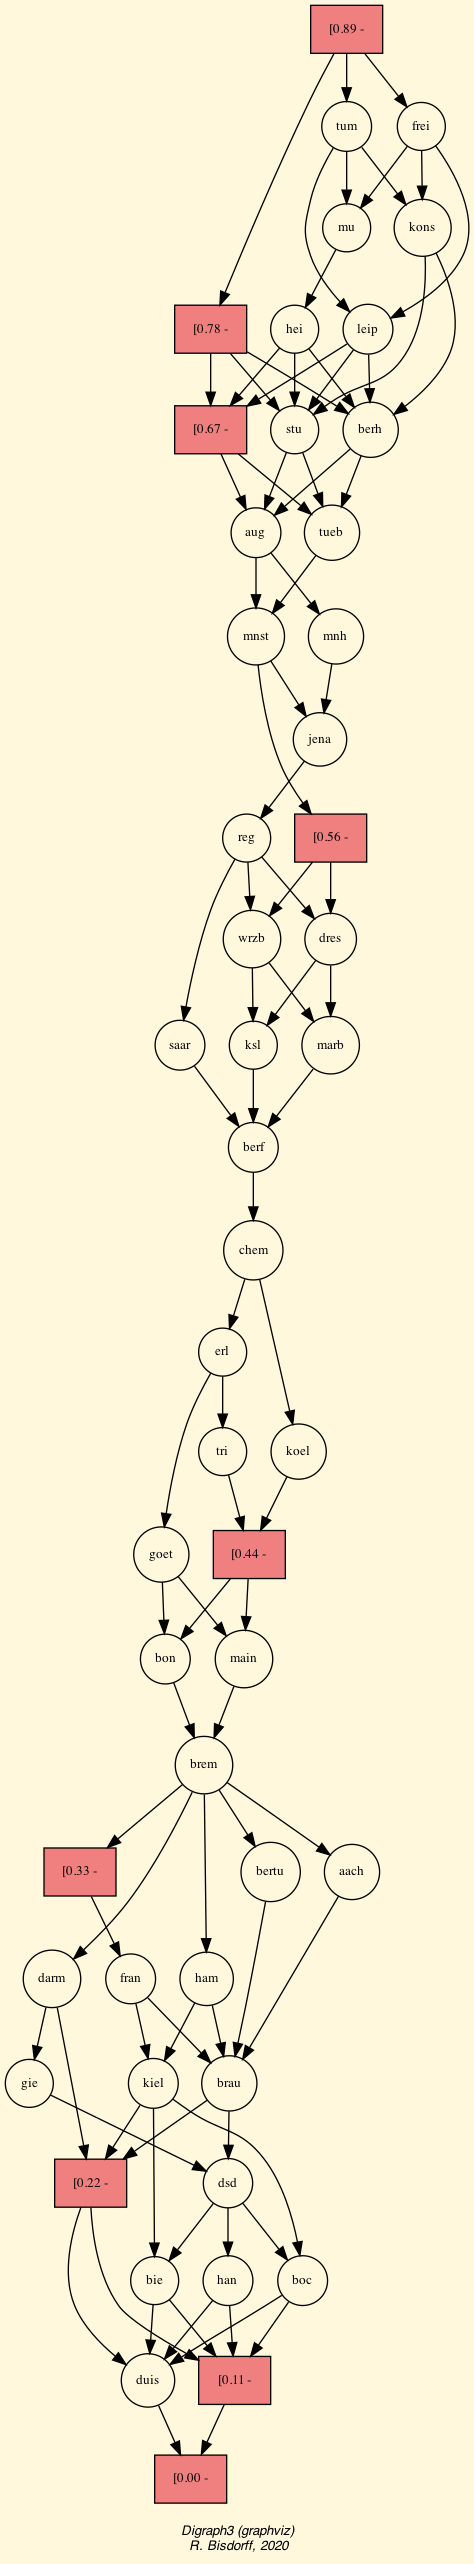
\includegraphics[width=4cm]{Figures/fusionResult.png}\\
\end{center}
\end{minipage}

\section{Inspecting the bipolar-valued outranking digraph}
\label{sec:14.2}

We say that University x \emph{outranks} (resp. \emph{is outranked by}) University $y$ in enrolment quality when there exists a majority (resp. only a minority) of valuated subjects showing an \emph{at least as good as} average enrolment quality score. To compute these outranking situations, we use the \texttt{BipolarOutrankingDigraph} constructor.

\begin{lstlisting}[caption={Computing 9-tiles of the enrolment quality scores per subject},label=list:14.4]
>>> from outrankingDigraphs import BipolarOutrankingDigraph
>>> dg = BipolarOutrankingDigraph(t) 
>>> dg
  *------- Object instance description ------*
    Instance class       : BipolarOutrankingDigraph
    Instance name        : rel_studentenSpiegel04
    Actions              : 41 (Universities)
    Criteria             : 15 (subjects)
    Size                 : 828 (outranking situations)
    Determinateness (%)  : 63.67
    Valuation domain     : [-1.00;1.00]
>>> dg.computeTransitivityDegree(Comments=True)
    Transitivity degree of digraph <rel_studentenSpiegel04>:
     triples x>y>z: 57837, closed: 30714, open: 27123
     (closed/triples) =  0.531
>>> dg.computeSymmetryDegree(Comments=True)
    Symmetry degree of digraph <rel_studentenSpiegel04>:
     arcs x>y: 793, symmetric: 35, asymmetric: 758
     symmetric/arcs =  0.044
\end{lstlisting}

The bipolar-valued outranking digraph $dg$ (see Listing \ref{list:14.4} Line 2), obtained with the given performance tableau $t$, shows 828 positively validated pairwise outranking situations (Line 9). Unfortunately, the transitivity of digraph $dg$ is far from being satisfied: nearly half of the transitive closure is missing (Line 15). Despite the rather large preference discrimination threshold (0.5) we have assumed (see Fig. \ref{fig:14.2}), there does not occur many indifference situations (Line 19).

We may furthermore check if there exists any \emph{cyclic} outranking situations.
    
\begin{lstlisting}[caption={Enumerating chordless outranking circuits},label=list:14.5]
>>> from outrankingDigraphs import BipolarOutrankingDigraph
>>> dg.computeChordlessCircuits()
>>> dg.showChordlessCircuits()
  *---- Chordless circuits ----*
   93 circuits.
    1:  ['aach','bie','darm','brau'] ,credibility : 0.067
    2:  ['aach','bertu','brau'] ,credibility : 0.200
    3:  ['aach','bertu','brem'] ,credibility : 0.067
    4:  ['aach','bertu','ham'] ,credibility : 0.200
    5:  ['aug','tri','marb'] ,credibility : 0.067
    6:  ['aug','jena','marb'] ,credibility : 0.067
    7:  ['aug','jena','koel'] ,credibility : 0.067
     ...
     ...
   29:  ['berh','kons','mu'] ,credibility : 0.133
     ...
     ...
   88:  ['main','mnh','marb'] ,credibility : 0.067
   89:  ['marb','saar','wrzb'] ,credibility : 0.067
   90:  ['marb','saar','reg'] ,credibility : 0.067
   91:  ['marb','saar','mnst'] ,credibility : 0.133
   92:  ['marb','saar','tri'] ,credibility : 0.067
   93:  ['mnh','mu','stu'] ,credibility : 0.133
 \end{lstlisting}

 Here we observe indeed 93 such outranking circuits, like: Berlin Humboldt $>$ Konstanz $>$ München $>$ Berlin Humboldt, supported by a $(0.133 + 1.0)/2 = 56.7\%$ majority of subjects Footnote[31] (see circuit 29 above). In the \Copeland ranking result shown in Fig. \ref{fig:14.4}, these Universities appear positioned respectively at ranks 10, 4 and 6. In the \NetFlows ranking result they would appear respectively at ranks 10, 6 and 5, thus inverting the positions of Konstanz and München. The occurrence in digraph $dg$ of so many outranking circuits makes thus \emph{doubtful} any \emph{forced} linear ranking, independently of the specific ranking rule we might have applied.

To effectively check the quality of our \Copeland rating-by-ranking result, we shall now compute a direct sorting into 9-tiles of the enrolment quality scores, without using any outranking digraph based ranking rule.

\section{Rating by quantiles sorting}
\label{sec:14.3}

In our case here, the Universities represent the decision actions: \emph{where to study}. We say now that University $x$ is sorted into the lower-closed 9-tile $q$ when the performance record of $x$ positively outranks the lower limit record of 9-tile $q$ and $x$ does not positively outrank the upper limit record of 9-tile $q$. 

\begin{lstlisting}[caption={Enumerating chordless outranking circuits},label=list:14.6,basicstyle=\scriptsize]
>>> lqr.showActionsSortingResult()
  Quantiles sorting result per decision action
  [0.33 - 0.44[: aach with credibility: 0.13 = min(0.13,0.27)
  [0.56 - 0.89[: aug with credibility: 0.13 = min(0.13,0.27)
  [0.44 - 0.67[: berf with credibility: 0.13 = min(0.13,0.20)
  [0.78 - 0.89[: berh with credibility: 0.13 = min(0.13,0.33)
  [0.22 - 0.44[: bertu with credibility: 0.20 = min(0.33,0.20)
  [0.11 - 0.22[: bie with credibility: 0.20 = min(0.33,0.20)
  [0.22 - 0.33[: boc with credibility: 0.07 = min(0.07,0.07)
  [0.44 - 0.56[: bon with credibility: 0.13 = min(0.20,0.13)
  [0.33 - 0.44[: brau with credibility: 0.07 = min(0.07,0.27)
  [0.33 - 0.44[: brem with credibility: 0.07 = min(0.07,0.07)
  [0.44 - 0.56[: chem with credibility: 0.07 = min(0.13,0.07)
  [0.22 - 0.56[: darm with credibility: 0.13 = min(0.13,0.13)
  [0.56 - 0.67[: dres with credibility: 0.27 = min(0.27,0.47)
  [0.22 - 0.33[: dsd with credibility: 0.07 = min(0.07,0.07)
  [0.00 - 0.11[: duis with credibility: 0.33 = min(0.73,0.33)
  [0.44 - 0.56[: erl with credibility: 0.13 = min(0.27,0.13)
  [0.22 - 0.44[: fran with credibility: 0.13 = min(0.13,0.33)
  [0.78 - <[: frei with credibility: 0.53 = min(0.53,1.00)
  [0.22 - 0.33[: gie with credibility: 0.13 = min(0.13,0.20)
  [0.33 - 0.44[: goet with credibility: 0.07 = min(0.47,0.07)
  [0.22 - 0.33[: ham with credibility: 0.07 = min(0.33,0.07)
  [0.11 - 0.22[: han with credibility: 0.20 = min(0.33,0.20)
  [0.78 - 0.89[: hei with credibility: 0.13 = min(0.13,0.27)
  [0.56 - 0.67[: jena with credibility: 0.07 = min(0.13,0.07)
  [0.33 - 0.44[: kiel with credibility: 0.20 = min(0.20,0.47)
  [0.44 - 0.56[: koel with credibility: 0.07 = min(0.27,0.07)
  [0.78 - <[: kons with credibility: 0.20 = min(0.20,1.00)
  [0.56 - 0.89[: ksl with credibility: 0.13 = min(0.13,0.40)
  [0.78 - 0.89[: leip with credibility: 0.07 = min(0.20,0.07)
  [0.44 - 0.56[: main with credibility: 0.07 = min(0.07,0.13)
  [0.56 - 0.67[: marb with credibility: 0.07 = min(0.07,0.07)
  [0.56 - 0.89[: mnh with credibility: 0.20 = min(0.20,0.27)
  [0.56 - 0.67[: mnst with credibility: 0.07 = min(0.20,0.07)
  [0.78 - 0.89[: mu with credibility: 0.13 = min(0.13,0.47)
  [0.56 - 0.67[: reg with credibility: 0.20 = min(0.20,0.27)
  [0.56 - 0.78[: saar with credibility: 0.13 = min(0.13,0.20)
  [0.78 - 0.89[: stu with credibility: 0.07 = min(0.13,0.07)
  [0.44 - 0.56[: tri with credibility: 0.07 = min(0.13,0.07)
  [0.67 - 0.78[: tueb with credibility: 0.13 = min(0.13,0.20)
  [0.89 - <[: tum with credibility: 0.13 = min(0.13,1.00)
  [0.56 - 0.67[: wrzb with credibility: 0.07 = min(0.20,0.07)
\end{lstlisting}

In the 9-tiles sorting result, shown in Listing \ref{list:14.6}, we notice for instance in Lines 3-4 that the RWTH Aachen is precisely rated into the 4th 9-tile ($[0.33 - 0.44[$), whereas the University Augsburg is less precisely rated conjointly into the $6^{th}$, the $7^{th}$ and the $8^{th}$ 9-tile ($[0.56 - 0.89[$). In Line 42, TU München appears best rated into the unique highest 9-tile ($[0.89 - <[$). All three rating results are supported by a $(0.07 + 1.0)/2 = 53.5\%$ majority of valuated subjects \footnote{Converted by a $+1.0$ shift and a $0.5 \times 100$ scale transform from a bipolar-valued credibility of $+0.07$ in $[-1.0, +1.0]$ to a majority (in \%) support.}. With the support of a $76.5\%$ majority of valuated subjects (Line 20), the apparent most confident rating result is the one of University Freiburg (see also Fig. \ref{fig:14.3} and Fig. \ref{fig:14.4}). 

We shall now lexicographically sort these individual rating results per University, by \emph{average} rated 9-tile limits and highest-rated upper 9-tile limit, into ordered, but not necessarily disjoint, enrolment quality quantiles.

\begin{lstlisting}
>>> lqr.showHTMLQuantilesSorting(strategy='average')
\end{lstlisting}

\begin{figure}[h]
\sidecaption
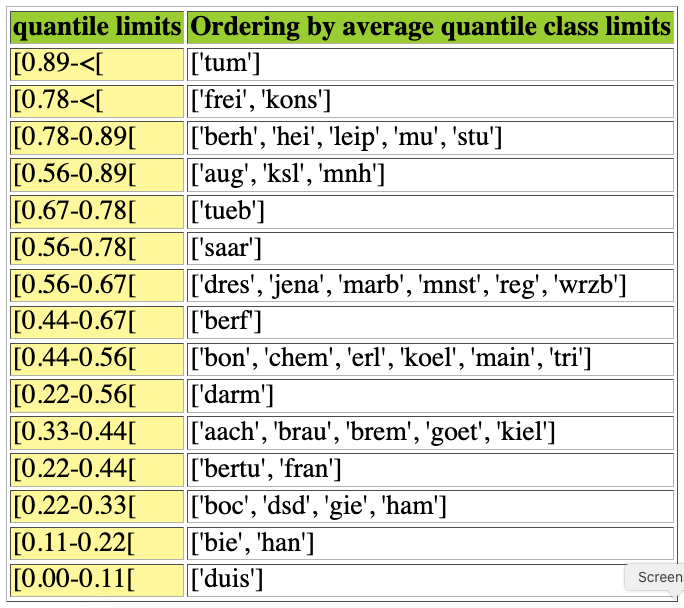
\includegraphics[width=7cm]{Figures/nineTilingOrdering.png}
\caption{The ranked 9-tiles rating-by-sorting result. We may notice that the Universities: Augsburg, Kaiserslautern, Mannheim and Tübingen, for instance, show in fact the same average rated 9-tiles score of $0.725$; yet, the rated upper 9-tile limit of Tuebingen reaches only $0.78$, whereas the one of the other Universities reaches $0.89$. Hence, Tuebingen is ranked below Augsburg, Kaiserslautern and Mannheim.}
\label{fig:14.6}       % Give a unique label
\end{figure}

With a special \emph{graphviz} drawing of the \texttt{LearnedQuantilesRatingDigraph} instance $lqr$, we may, without requiring any specific ordering strategy, as well illustrate our 9-tiles rating-by-sorting result.

\begin{lstlisting}
>>> lqr.exportRatingBySortingGraphViz(\
...           'nineTilingDrawing',graphSize='12,12')
  *---- exporting a dot file for GraphViz tools --*
   Exporting to nineTilingDrawing.dot
   dot -Grankdir=TB -Tpng nineTilingDrawing.dot\
                     -o nineTilingDrawing.png
\end{lstlisting}

\begin{figure}[h]
%\sidecaption
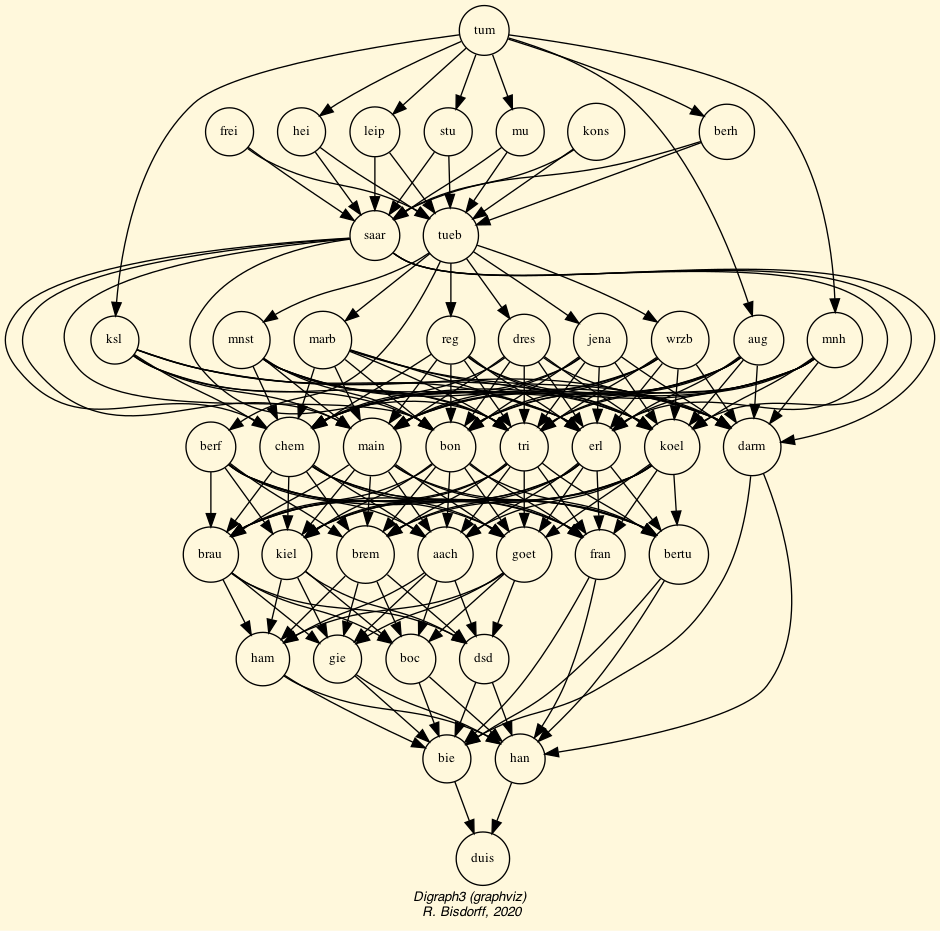
\includegraphics[width=12cm]{Figures/nineTilingDrawing.png}
\caption{Graphviz drawing of the 9-tiles sorting digraph.}
\label{fig:14.7}       % Give a unique label
\end{figure}

In Fig. \ref{fig:14.7} we actually see the \emph{skeleton} (transitive closure removed) of a partial order, where an oriented arc is drawn between Universities x and y when their 9-tiles sorting results are disjoint and the one of x is higher rated than the one of $y$. The rating for TU München (see Listing \ref{list:14.6} Lines 45), for instance, is disjoint and higher rated than the one of the Universities Freiburg and Konstanz (Lines 23, 32). And, both the ratings of Feiburg and Konstanz are, however, not disjoint from the one, for instance, of the Universty of Stuttgart (Line 42).

The partial ranking, shown in Fug. \ref{fig:14.7}, is in fact independent of any ordering strategy: - \emph{average}, - \emph{optimistic} - \emph{pessimistic}, of overlapping 9-tiles sorting results, and confirms that the same Universities as with the previous rating-by-ranking approach, namely TU München, Freiburg, Konstanz, Stuttgart, Berlin Humboldt, Heidelberg and Leipzig appear top-rated. Similarly, the Universities of Duisburg, Bielefeld, Hanover, Bochum, Giessen, Düsseldorf and Hamburg give the lowest-rated group. The midfield here is again consisting of more or less the same Universities as the one observed in the previous rating-by-ranking approach (see Listing \ref{list:14.3}).

In the end, both the \Copeland rating-by-ranking, as well as the rating-by-sorting approach give luckily, in our case study here, very similar results. The first approach, with its \emph{forced} linear ranking, determines on the one hand, precise enrolment quality equivalence classes; a result, depending potentially a lot on the actually applied ranking rule. The rating-by-sorting approach, on the other hand, only determines for each University a less precise but prudent rating of its individual enrolment quality, furthermore supported by a known majority of performance criteria significance; a somehow fairer and robuster result, but, much less evident for easily comparing the apparent enrolment quality among Universities. Contradictorily, or sparsely valuated Universities, for instance, will appear trivially rated into a large midfield of adjacent 9-tiles.

Let us conclude by saying that we prefer this latter rating-by-sorting approach; perhaps impreciser, due the case given, to missing and contradictory performance data; yet, well grounded in a powerful bipolar-valued logical and espistemic framework.
 
